% Options for packages loaded elsewhere
\PassOptionsToPackage{unicode}{hyperref}
\PassOptionsToPackage{hyphens}{url}
\PassOptionsToPackage{dvipsnames,svgnames,x11names}{xcolor}
\documentclass[
]{article}
\usepackage{xcolor}
\usepackage[margin=1in]{geometry}
\usepackage{amsmath,amssymb}
\setcounter{secnumdepth}{5}
\usepackage{iftex}
\ifPDFTeX
  \usepackage[T1]{fontenc}
  \usepackage[utf8]{inputenc}
  \usepackage{textcomp} % provide euro and other symbols
\else % if luatex or xetex
  \usepackage{unicode-math} % this also loads fontspec
  \defaultfontfeatures{Scale=MatchLowercase}
  \defaultfontfeatures[\rmfamily]{Ligatures=TeX,Scale=1}
\fi
\usepackage{lmodern}
\ifPDFTeX\else
  % xetex/luatex font selection
\fi
% Use upquote if available, for straight quotes in verbatim environments
\IfFileExists{upquote.sty}{\usepackage{upquote}}{}
\IfFileExists{microtype.sty}{% use microtype if available
  \usepackage[]{microtype}
  \UseMicrotypeSet[protrusion]{basicmath} % disable protrusion for tt fonts
}{}
\makeatletter
\@ifundefined{KOMAClassName}{% if non-KOMA class
  \IfFileExists{parskip.sty}{%
    \usepackage{parskip}
  }{% else
    \setlength{\parindent}{0pt}
    \setlength{\parskip}{6pt plus 2pt minus 1pt}}
}{% if KOMA class
  \KOMAoptions{parskip=half}}
\makeatother
\usepackage{color}
\usepackage{fancyvrb}
\newcommand{\VerbBar}{|}
\newcommand{\VERB}{\Verb[commandchars=\\\{\}]}
\DefineVerbatimEnvironment{Highlighting}{Verbatim}{commandchars=\\\{\}}
% Add ',fontsize=\small' for more characters per line
\newenvironment{Shaded}{}{}
\newcommand{\AlertTok}[1]{\textcolor[rgb]{1.00,0.00,0.00}{\textbf{#1}}}
\newcommand{\AnnotationTok}[1]{\textcolor[rgb]{0.38,0.63,0.69}{\textbf{\textit{#1}}}}
\newcommand{\AttributeTok}[1]{\textcolor[rgb]{0.49,0.56,0.16}{#1}}
\newcommand{\BaseNTok}[1]{\textcolor[rgb]{0.25,0.63,0.44}{#1}}
\newcommand{\BuiltInTok}[1]{\textcolor[rgb]{0.00,0.50,0.00}{#1}}
\newcommand{\CharTok}[1]{\textcolor[rgb]{0.25,0.44,0.63}{#1}}
\newcommand{\CommentTok}[1]{\textcolor[rgb]{0.38,0.63,0.69}{\textit{#1}}}
\newcommand{\CommentVarTok}[1]{\textcolor[rgb]{0.38,0.63,0.69}{\textbf{\textit{#1}}}}
\newcommand{\ConstantTok}[1]{\textcolor[rgb]{0.53,0.00,0.00}{#1}}
\newcommand{\ControlFlowTok}[1]{\textcolor[rgb]{0.00,0.44,0.13}{\textbf{#1}}}
\newcommand{\DataTypeTok}[1]{\textcolor[rgb]{0.56,0.13,0.00}{#1}}
\newcommand{\DecValTok}[1]{\textcolor[rgb]{0.25,0.63,0.44}{#1}}
\newcommand{\DocumentationTok}[1]{\textcolor[rgb]{0.73,0.13,0.13}{\textit{#1}}}
\newcommand{\ErrorTok}[1]{\textcolor[rgb]{1.00,0.00,0.00}{\textbf{#1}}}
\newcommand{\ExtensionTok}[1]{#1}
\newcommand{\FloatTok}[1]{\textcolor[rgb]{0.25,0.63,0.44}{#1}}
\newcommand{\FunctionTok}[1]{\textcolor[rgb]{0.02,0.16,0.49}{#1}}
\newcommand{\ImportTok}[1]{\textcolor[rgb]{0.00,0.50,0.00}{\textbf{#1}}}
\newcommand{\InformationTok}[1]{\textcolor[rgb]{0.38,0.63,0.69}{\textbf{\textit{#1}}}}
\newcommand{\KeywordTok}[1]{\textcolor[rgb]{0.00,0.44,0.13}{\textbf{#1}}}
\newcommand{\NormalTok}[1]{#1}
\newcommand{\OperatorTok}[1]{\textcolor[rgb]{0.40,0.40,0.40}{#1}}
\newcommand{\OtherTok}[1]{\textcolor[rgb]{0.00,0.44,0.13}{#1}}
\newcommand{\PreprocessorTok}[1]{\textcolor[rgb]{0.74,0.48,0.00}{#1}}
\newcommand{\RegionMarkerTok}[1]{#1}
\newcommand{\SpecialCharTok}[1]{\textcolor[rgb]{0.25,0.44,0.63}{#1}}
\newcommand{\SpecialStringTok}[1]{\textcolor[rgb]{0.73,0.40,0.53}{#1}}
\newcommand{\StringTok}[1]{\textcolor[rgb]{0.25,0.44,0.63}{#1}}
\newcommand{\VariableTok}[1]{\textcolor[rgb]{0.10,0.09,0.49}{#1}}
\newcommand{\VerbatimStringTok}[1]{\textcolor[rgb]{0.25,0.44,0.63}{#1}}
\newcommand{\WarningTok}[1]{\textcolor[rgb]{0.38,0.63,0.69}{\textbf{\textit{#1}}}}
\usepackage{longtable,booktabs,array}
\newcounter{none} % for unnumbered tables
\usepackage{calc} % for calculating minipage widths
% Correct order of tables after \paragraph or \subparagraph
\usepackage{etoolbox}
\makeatletter
\patchcmd\longtable{\par}{\if@noskipsec\mbox{}\fi\par}{}{}
\makeatother
% Allow footnotes in longtable head/foot
\IfFileExists{footnotehyper.sty}{\usepackage{footnotehyper}}{\usepackage{footnote}}
\makesavenoteenv{longtable}
\usepackage{graphicx}
\makeatletter
\newsavebox\pandoc@box
\newcommand*\pandocbounded[1]{% scales image to fit in text height/width
  \sbox\pandoc@box{#1}%
  \Gscale@div\@tempa{\textheight}{\dimexpr\ht\pandoc@box+\dp\pandoc@box\relax}%
  \Gscale@div\@tempb{\linewidth}{\wd\pandoc@box}%
  \ifdim\@tempb\p@<\@tempa\p@\let\@tempa\@tempb\fi% select the smaller of both
  \ifdim\@tempa\p@<\p@\scalebox{\@tempa}{\usebox\pandoc@box}%
  \else\usebox{\pandoc@box}%
  \fi%
}
% Set default figure placement to htbp
\def\fps@figure{htbp}
\makeatother
\setlength{\emergencystretch}{3em} % prevent overfull lines
\providecommand{\tightlist}{%
  \setlength{\itemsep}{0pt}\setlength{\parskip}{0pt}}
\usepackage{float}
\usepackage{booktabs}
\usepackage{amsmath}
\floatplacement{figure}{H}
\usepackage{bookmark}
\IfFileExists{xurl.sty}{\usepackage{xurl}}{} % add URL line breaks if available
\urlstyle{same}
% fallback for those not using the hyperref driver hyperxmp:
\makeatletter
\@ifundefined{xmpquote}{\newcommand{\xmpquote}[1]{#1}}{}
\makeatother
\hypersetup{
  pdftitle={FHSS Transceiver with Hop Synchronization and Partial-Band Interference},
  pdfauthor={Wireless Communication Class Project},
  colorlinks=true,
  linkcolor={blue},
  filecolor={Maroon},
  citecolor={Blue},
  urlcolor={Blue},
  pdfcreator={LaTeX via pandoc}}

\title{FHSS Transceiver with Hop Synchronization and Partial-Band
Interference}
\usepackage{etoolbox}
\makeatletter
\providecommand{\subtitle}[1]{% add subtitle to \maketitle
  \apptocmd{\@title}{\par {\large #1 \par}}{}{}
}
\makeatother
\subtitle{Wireless Communication Project Report}
\author{Wireless Communication Class Project}
\date{31 August 2026}

\begin{document}
\maketitle

{
\setcounter{tocdepth}{3}
\tableofcontents
}
\section{Abstract}\label{abstract}

This project designs and evaluates a frequency-hopping spread-spectrum
(FHSS) transceiver in base MATLAB. A framed BPSK payload is transmitted
over eight pseudo-random carrier offsets while a jammer occupies only
part of the hopping band. The receiver performs preamble-assisted hop
timing and hopping-code acquisition, dehopping, coherent BPSK detection,
frame synchronization, and CRC-16 checking. Reliability is measured
using payload bit error rate (BER), packet error rate (PER), and
synchronization probability. Experiments vary jammer occupancy, hop
rate, hopping mismatch, and receiver dwell-rate error, then compare FHSS
with an equal-power fixed-frequency BPSK link. The complete experiment
is deterministic and requires no MATLAB toolboxes.

\section{Objectives}\label{objectives}

The work addresses four objectives:

\begin{enumerate}
\def\labelenumi{\arabic{enumi}.}
\tightlist
\item
  Synthesize and visualize a reproducible framed FHSS waveform.
\item
  Model AWGN and a configurable partial-band interferer.
\item
  recover the payload through hop and frame synchronization, dehopping,
  BPSK demodulation, and CRC validation.
\item
  Quantify BER/PER and make an engineering recommendation for hop-set
  size and hop rate.
\end{enumerate}

The implementation is a complex low-intermediate-frequency equivalent of
a nominal 2.4 GHz radio. Directly sampling a 2.4 GHz carrier is
unnecessary because frequency translation preserves the modulation and
interference relationships being studied.

\section{System Design}\label{system-design}

\subsection{Transmitter and receiver
architecture}\label{transmitter-and-receiver-architecture}

\begin{figure}
\centering
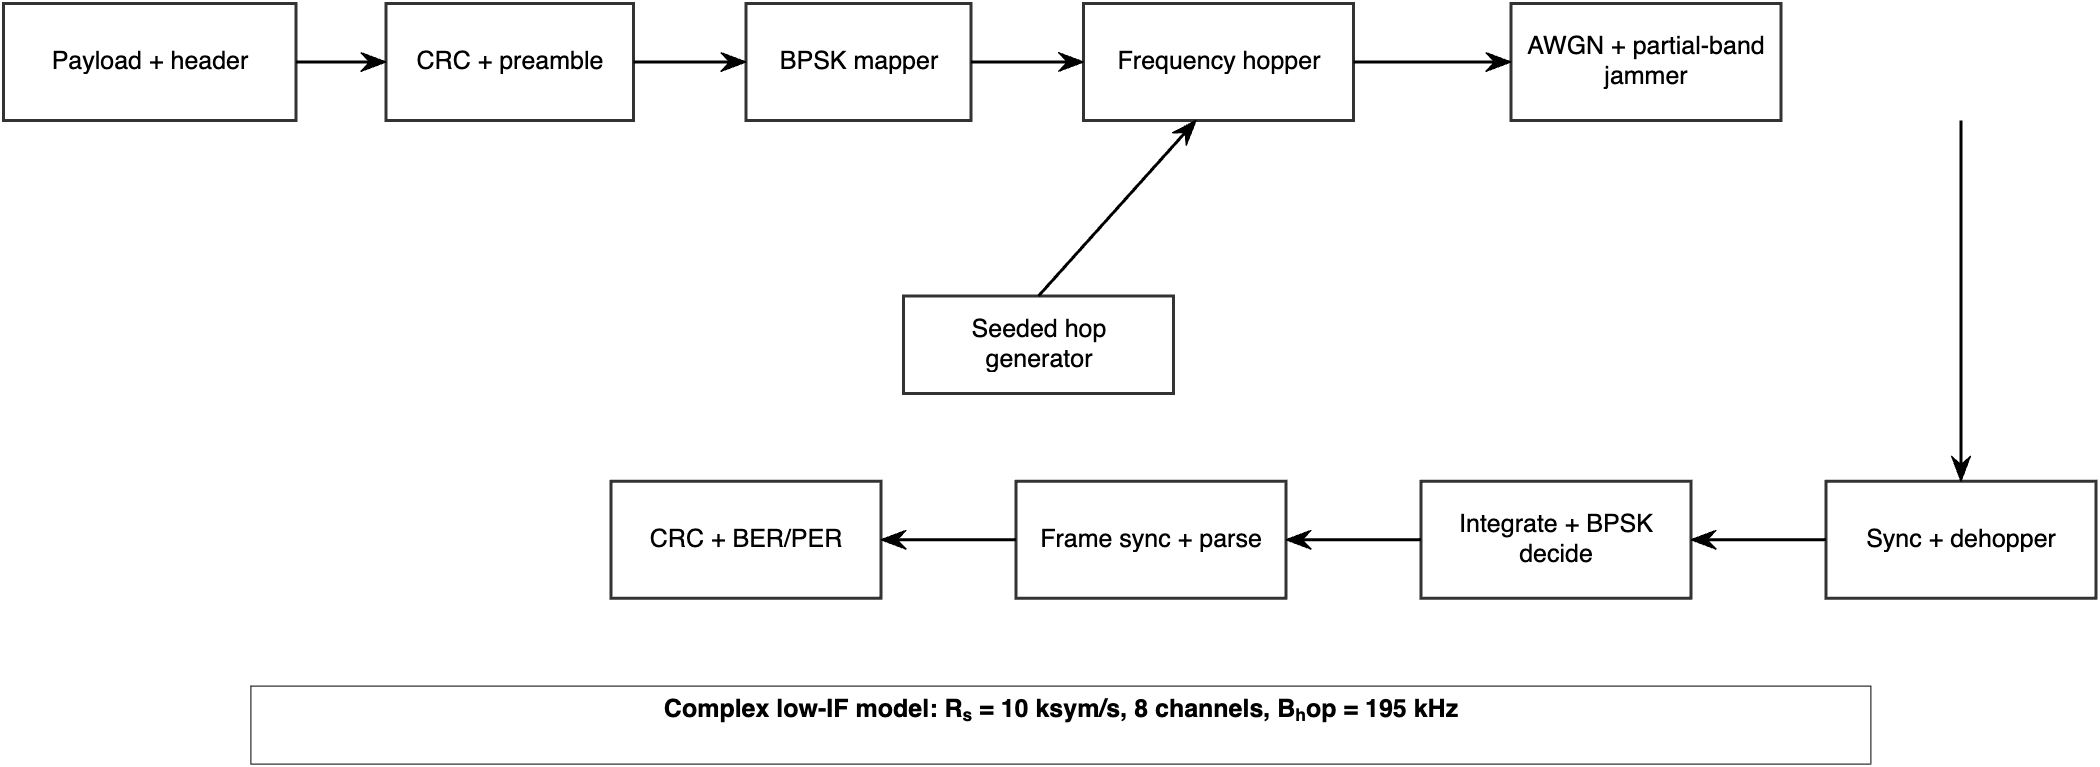
\includegraphics[width=0.96\linewidth,height=\textheight,keepaspectratio,alt={FHSS transmitter, channel, and receiver processing chain.}]{figures/tx_rx_block_diagram.png}
\caption{FHSS transmitter, channel, and receiver processing chain.}
\end{figure}

The transmitter appends a fixed synchronization word and CRC to each
payload, maps the bits to BPSK symbols, and mixes each dwell interval to
a carrier selected by a shared pseudo-random generator. The receiver
evaluates timing and hopping-code candidates with the known preamble,
reconstructs the winning carrier schedule, dehops the samples, and uses
integrate-and-dump symbol decisions. A frame is accepted only if
preamble detection and CRC validation succeed.

\subsection{Frame and modulation}\label{frame-and-modulation}

The fixed-length 320-bit frame is shown in Table 1. The CRC covers the
header and payload but not the preamble.

\begin{longtable}[]{@{}lrl@{}}
\caption{Frame format}\label{tbl:frame}\tabularnewline
\toprule\noalign{}
Field & Length & Purpose \\
\midrule\noalign{}
\endfirsthead
\toprule\noalign{}
Field & Length & Purpose \\
\midrule\noalign{}
\endhead
\bottomrule\noalign{}
\endlastfoot
Synchronization word & 32 bits & Hexadecimal \texttt{0x1ACFFC1D} \\
Frame counter & 16 bits & Packet identification \\
Payload & 256 bits & BER measurement data \\
CRC-16 & 16 bits & Packet acceptance \\
\end{longtable}

CRC-16/CCITT-FALSE uses polynomial \(0x1021\), initial state \(0xFFFF\),
no input/output reflection, and no final XOR. Its standard
\texttt{123456789} check value is \(0x29B1\).

BPSK mapping is

\[
a_k = 1-2b_k,
\]

where \(b_k\in\{0,1\}\) and \(a_k\in\{+1,-1\}\). Rectangular pulse
shaping gives 50 samples/symbol at \(R_s=10\) ksymbol/s and \(F_s=500\)
ksample/s. Transmit power is normalized to unity.

\subsection{Hopping design and
bandwidth}\label{hopping-design-and-bandwidth}

The eight low-IF carrier offsets are

\[
[-87.5,-62.5,-37.5,-12.5,12.5,37.5,62.5,87.5]\ \text{kHz}.
\]

They are separated by \(\Delta f=25\) kHz. Rectangular BPSK has an
approximate null-to-null occupied width \(B_\text{ch}=2R_s=20\) kHz,
leaving a 5 kHz separation margin. The total hopping bandwidth is

\[
B_\text{hop}=(N-1)\Delta f+B_\text{ch}
            =(8-1)(25)+20=195\ \text{kHz}.
\]

For \(N_s\) symbols per hop,

\[
T_d=\frac{N_s}{R_s}, \qquad R_h=\frac{1}{T_d}=\frac{R_s}{N_s}.
\]

\begin{longtable}[]{@{}rrrr@{}}
\caption{Hopping configurations}\label{tbl:hops}\tabularnewline
\toprule\noalign{}
Symbols/hop & Dwell time & Hop rate & Hops/frame \\
\midrule\noalign{}
\endfirsthead
\toprule\noalign{}
Symbols/hop & Dwell time & Hop rate & Hops/frame \\
\midrule\noalign{}
\endhead
\bottomrule\noalign{}
\endlastfoot
16 & 1.6 ms & 625 hops/s & 20 \\
8 & 0.8 ms & 1,250 hops/s & 40 \\
4 & 0.4 ms & 2,500 hops/s & 80 \\
\end{longtable}

The hopping generator uses a fixed Mersenne Twister seed. Successive
random permutations of all eight channels ensure balanced use while
retaining a reproducible pseudo-random order.

\begin{figure}
\centering
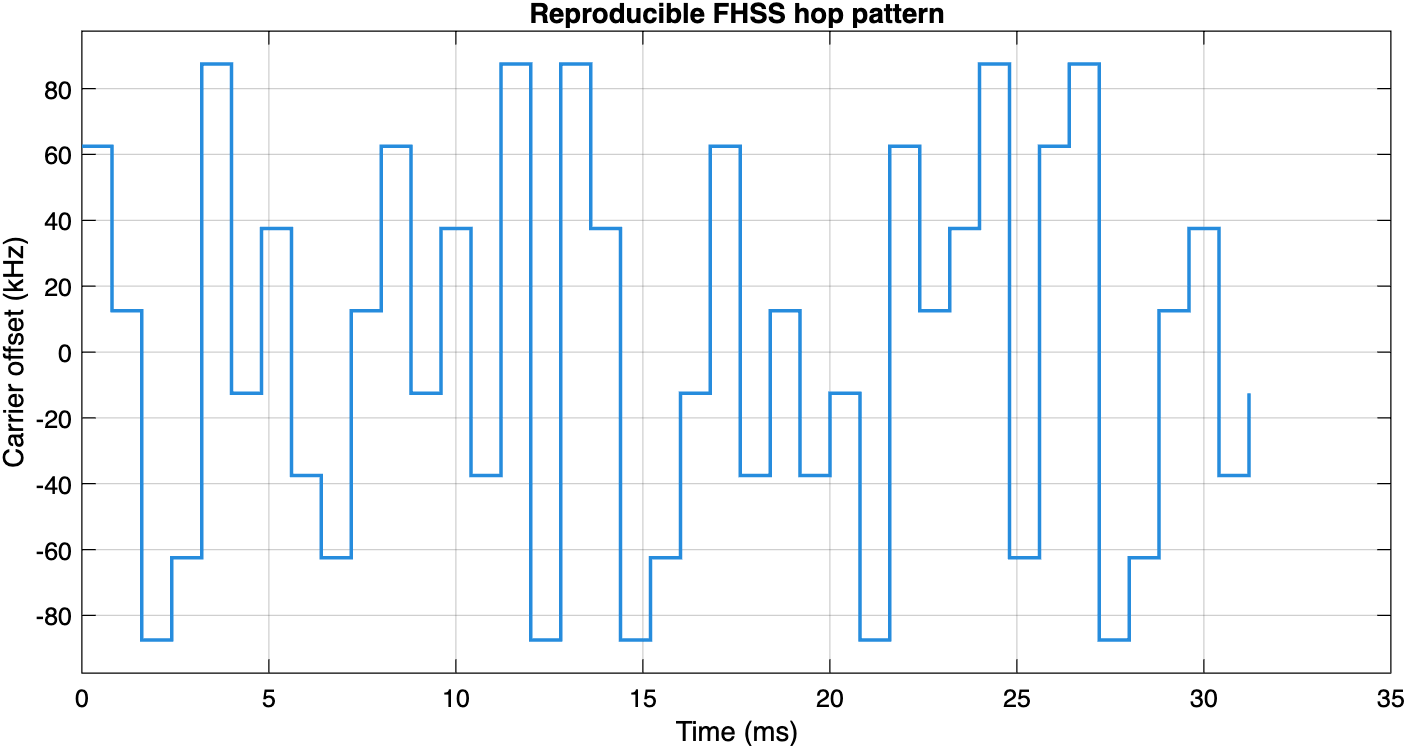
\includegraphics[width=0.88\linewidth,height=\textheight,keepaspectratio,alt={Baseline pseudo-random carrier sequence.}]{figures/hop_pattern.png}
\caption{Baseline pseudo-random carrier sequence.}
\end{figure}

\begin{figure}
\centering
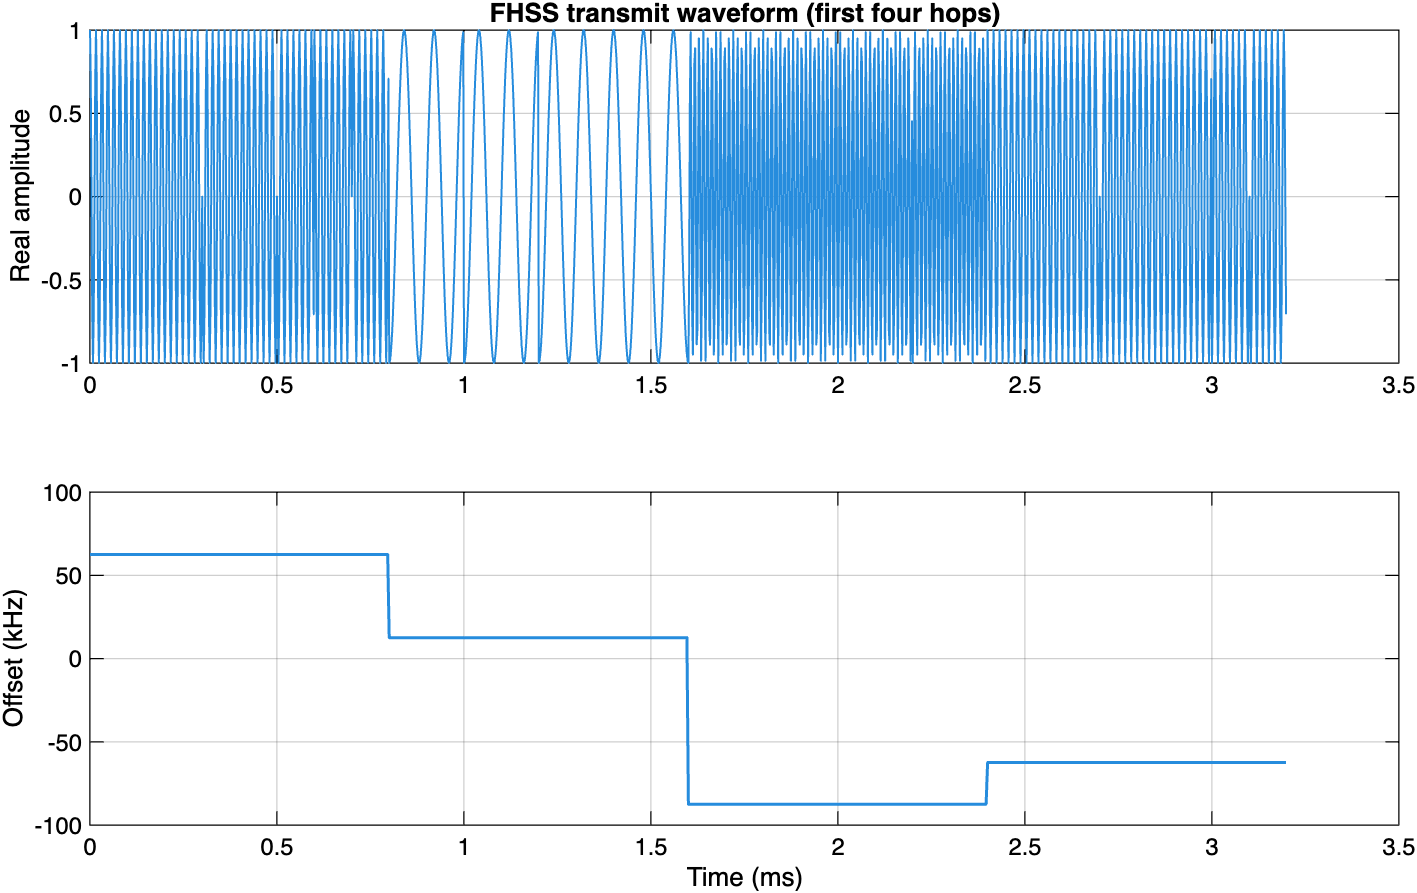
\includegraphics[width=0.92\linewidth,height=\textheight,keepaspectratio,alt={Real transmit waveform and instantaneous hop offset.}]{figures/transmit_waveform.png}
\caption{Real transmit waveform and instantaneous hop offset.}
\end{figure}

\section{Channel and Interference
Model}\label{channel-and-interference-model}

Complex AWGN is scaled from \(E_b/N_0\). For unit BPSK amplitude and
\(L\) samples/symbol, the complex sample-noise variance is

\[
\sigma_n^2=\frac{L}{10^{(E_b/N_0)_\text{dB}/10}},
\]

which produces a real decision-noise variance of \(1/(2E_b/N_0)\) after
integrate-and-dump detection. Without interference, the expected
coherent BPSK result is

\[
P_b=Q\!\left(\sqrt{2E_b/N_0}\right)
   =\frac{1}{2}\operatorname{erfc}\!\left(\sqrt{E_b/N_0}\right).
\]

The partial-band jammer occupies a contiguous central subset of the hop
channels. Independent complex Gaussian symbols are rectangularly shaped
and translated to every occupied jammer channel. Aggregate jammer power
is fixed at \(J/S=10\) dB and divided equally between occupied channels.
Consequently, increasing occupancy changes both the probability of a hop
collision and jammer power per occupied channel; it does not silently
increase total jammer power.

\begin{figure}
\centering
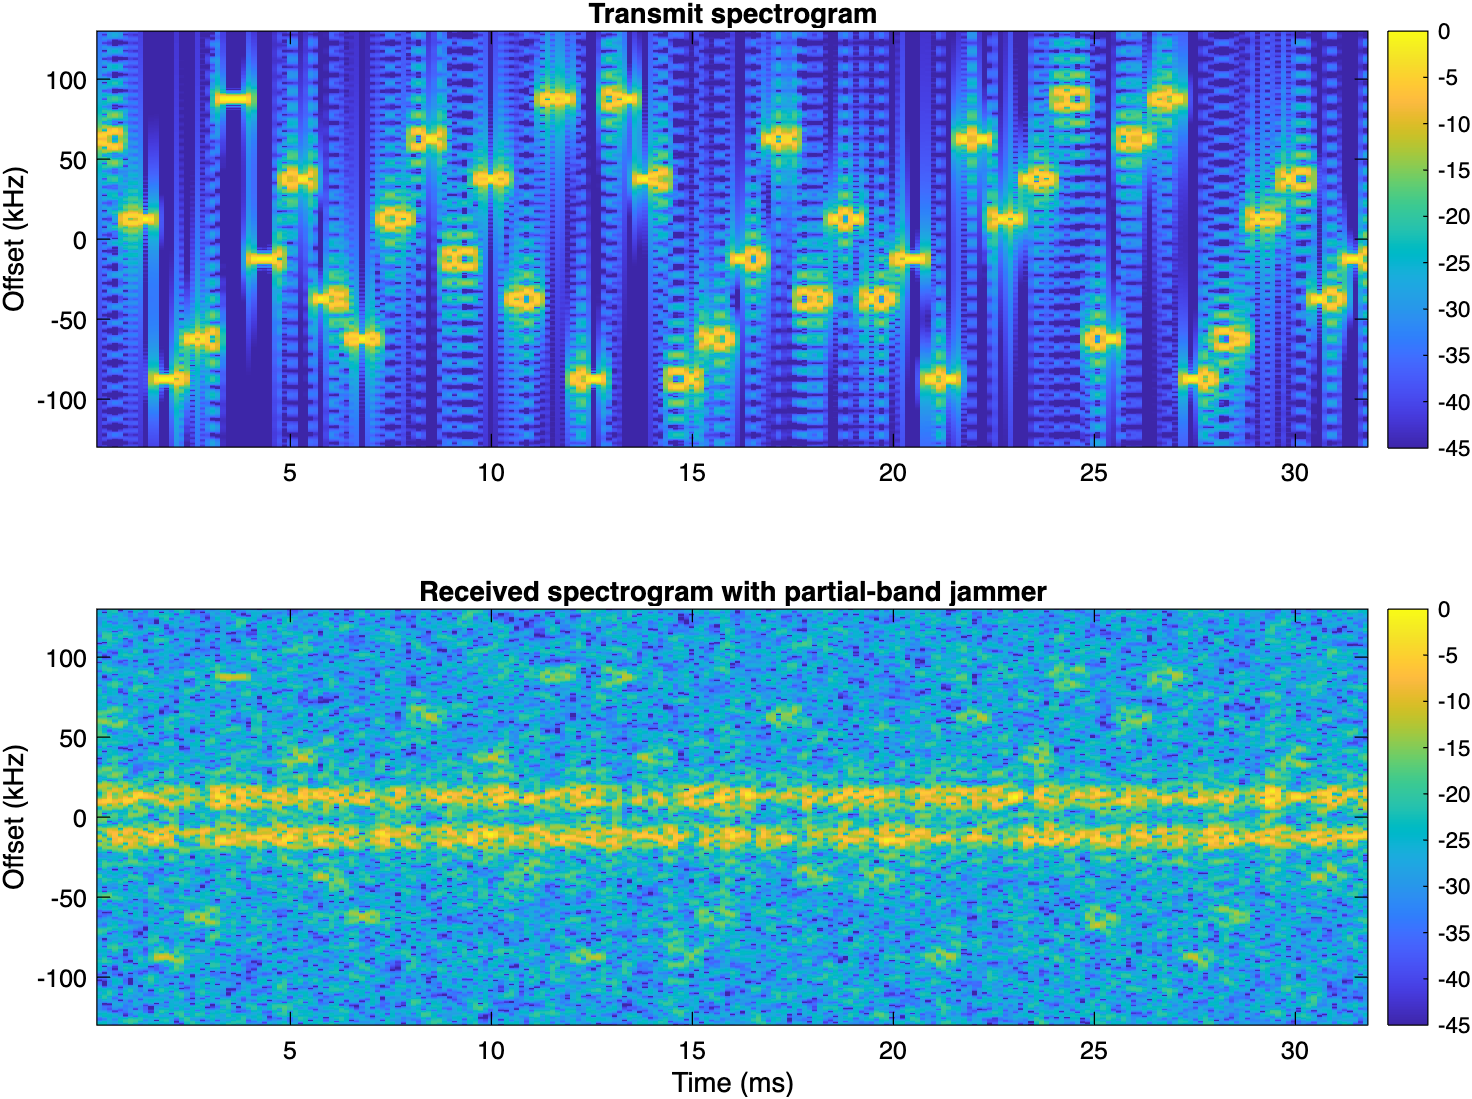
\includegraphics[width=0.96\linewidth,height=\textheight,keepaspectratio,alt={Transmit and received spectrograms for 25\% jammer occupancy.}]{figures/spectrograms.png}
\caption{Transmit and received spectrograms for 25\% jammer occupancy.}
\end{figure}

\begin{figure}
\centering
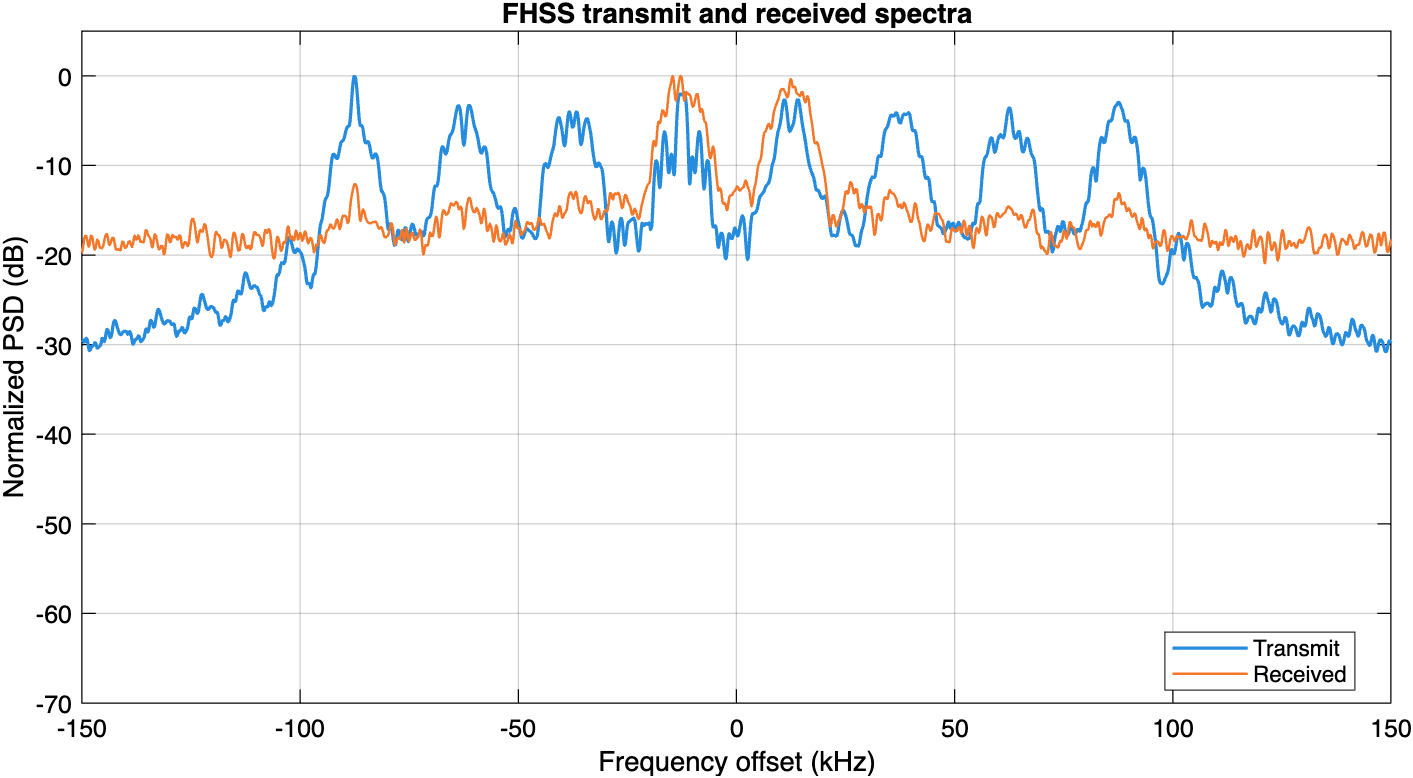
\includegraphics[width=0.9\linewidth,height=\textheight,keepaspectratio,alt={Normalized transmit and received power spectra.}]{figures/transmit_receive_spectrum.png}
\caption{Normalized transmit and received power spectra.}
\end{figure}

\section{Receiver Synchronization}\label{receiver-synchronization}

The receiver knows the hop set, seed, symbol rate, and nominal dwell
duration but not the exact packet boundary or hopping-code phase. It
searches code offsets from \(-8\) through \(+8\) hops and evaluates
every sample timing within one dwell. The exhaustive timing search
avoids carrier-dependent phase ambiguity that can make a symbol-spaced
coarse search select the wrong refinement region.

For a candidate soft preamble vector \(\mathbf{y}\) and known bipolar
preamble \(\mathbf{p}\), the acquisition metric is normalized
correlation:

\[
M=\frac{\mathbf{y}^{T}\mathbf{p}}
        {\sqrt{(\mathbf{y}^{T}\mathbf{y})(\mathbf{p}^{T}\mathbf{p})}}.
\]

Acquisition requires \(M\geq0.70\) and at least 28 of 32 correct hard
preamble decisions. After dehopping, the receiver performs another
Hamming-distance preamble search, extracts the frame, and verifies CRC.
A synchronization failure or CRC failure counts as a packet error. BER
is calculated only from the 256 payload bits.

Deliberate impairment tests force a one-hop sequence offset or receiver
dwell-rate errors from \(-2\%\) through \(+2\%\). Fractional receiver
hop boundaries are accumulated before rounding so that the
implementation does not add a systematic per-hop rounding bias.

\section{Experiment Method}\label{experiment-method}

The BER/PER grid uses \(E_b/N_0=0:2:14\) dB, jammer occupancies of 0\%,
12.5\%, 25\%, and 50\%, and all three hop rates. Every operating point
uses at least 250 packets and stops after 100 packet errors or 2,000
packets. Wilson 95\% confidence intervals quantify Monte Carlo
uncertainty.

The complete sample-domain waveform is used for the aligned-link BER/PER
grid, synchronization, code-phase error, and hop-rate mismatch. A fast
symbol-domain model is retained for the fixed-frequency decision-level
comparison. Selected operating points quantify the difference between
that abstraction and the waveform model under asynchronous partial-band
interference.

The fixed-frequency comparison preserves BPSK symbol rate and average
transmit power. It includes fixed jammed and clean carriers and a fixed
channel chosen uniformly per packet, preventing a single favorable
carrier choice from being mistaken for general fixed-link performance.

\section{Results and Analysis}\label{results-and-analysis}

\begin{figure}
\centering
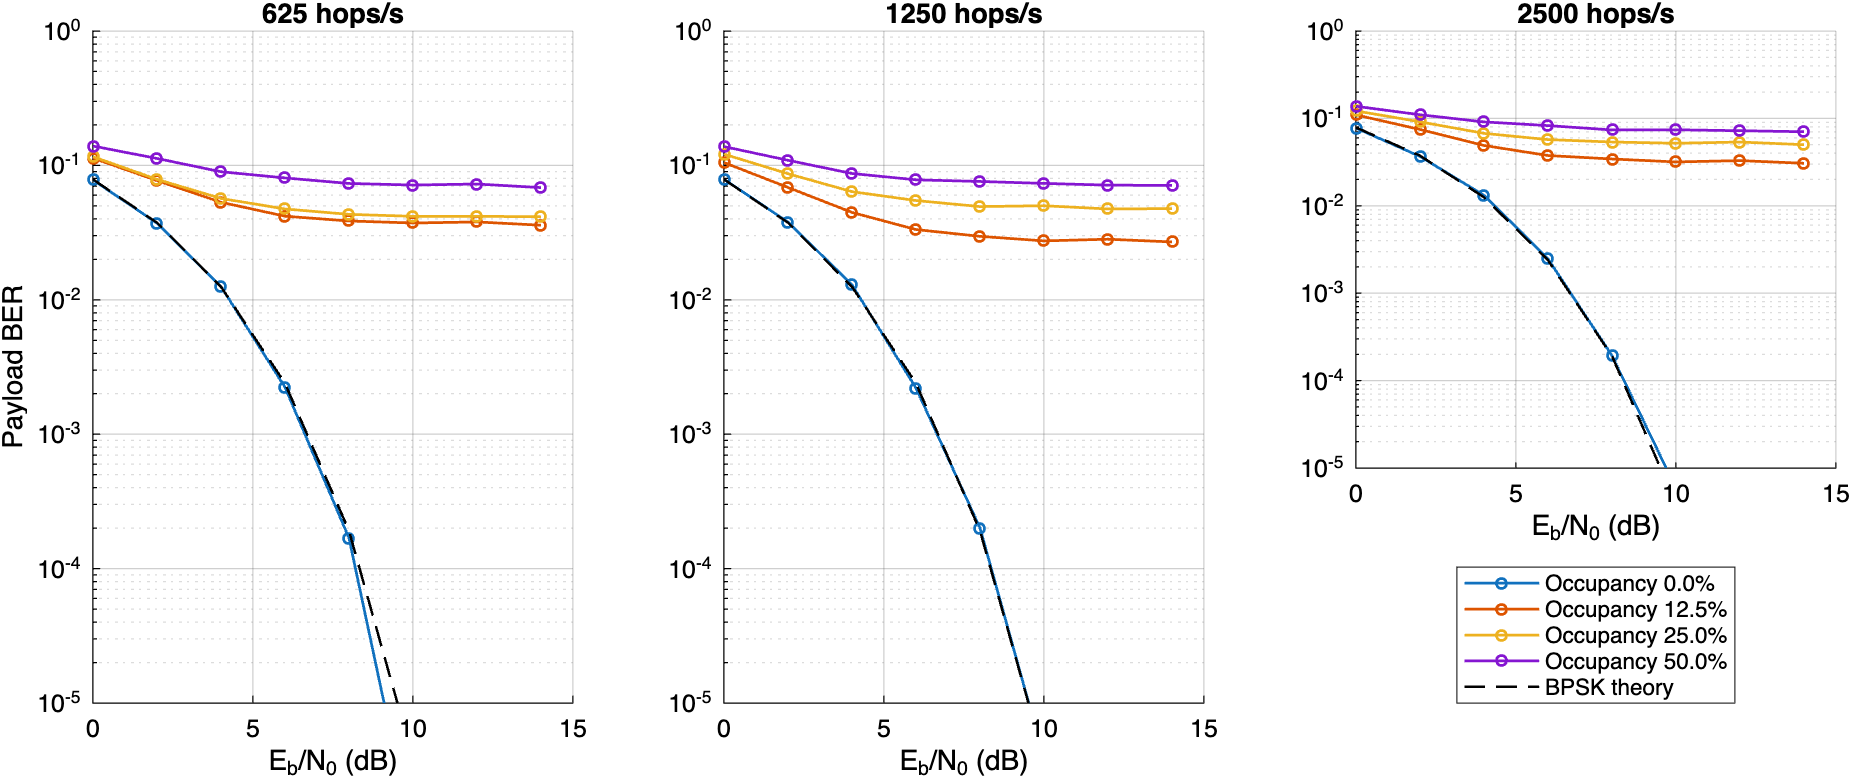
\includegraphics[width=1\linewidth,height=\textheight,keepaspectratio,alt={BER across jammer occupancy and hop rate. The dashed reference is theoretical jammer-free BPSK.}]{figures/ber_occupancy_hoprate.png}
\caption{BER across jammer occupancy and hop rate. The dashed reference
is theoretical jammer-free BPSK.}
\end{figure}

\begin{figure}
\centering
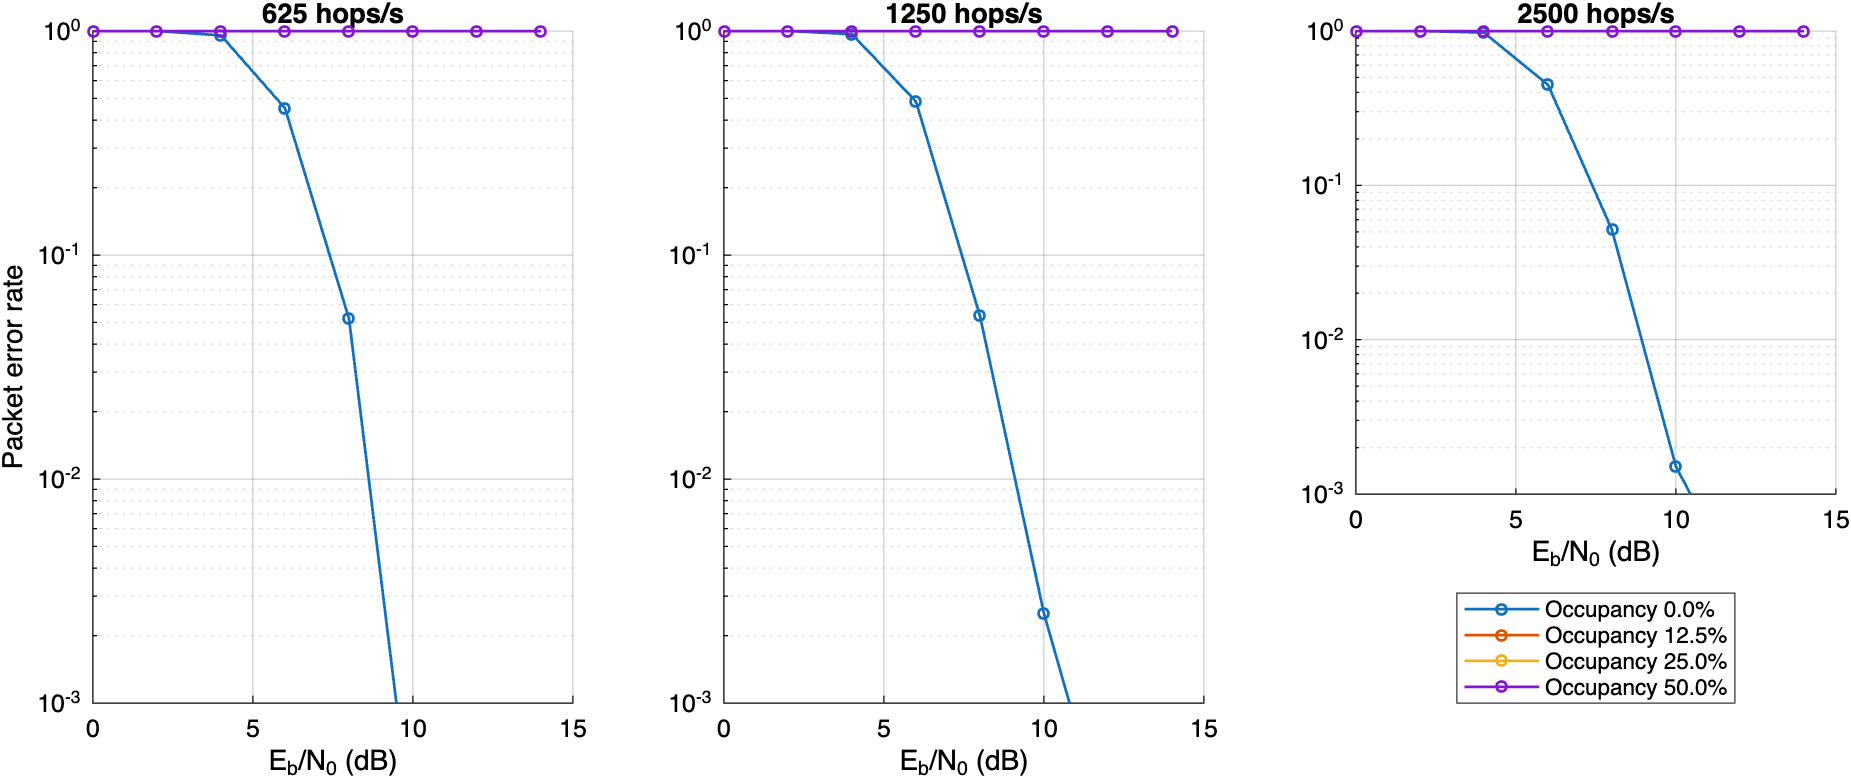
\includegraphics[width=1\linewidth,height=\textheight,keepaspectratio,alt={PER across jammer occupancy and hop rate.}]{figures/per_occupancy_hoprate.png}
\caption{PER across jammer occupancy and hop rate.}
\end{figure}

\begin{figure}
\centering
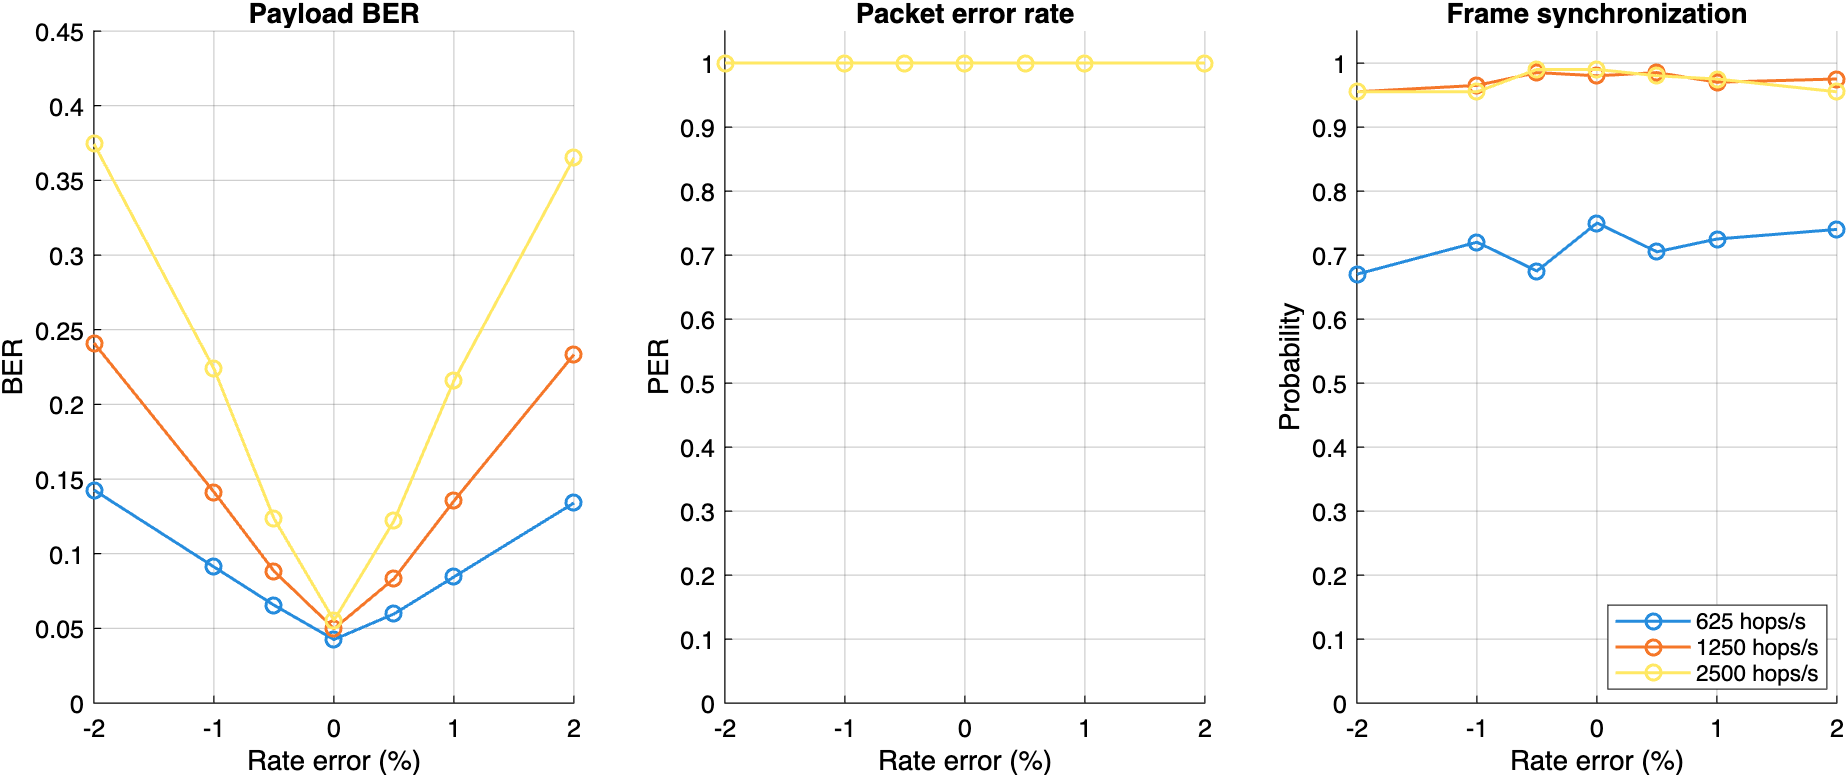
\includegraphics[width=1\linewidth,height=\textheight,keepaspectratio,alt={BER, PER, and synchronization sensitivity to receiver hop-rate mismatch.}]{figures/hop_rate_mismatch.png}
\caption{BER, PER, and synchronization sensitivity to receiver hop-rate
mismatch.}
\end{figure}

\begin{figure}
\centering
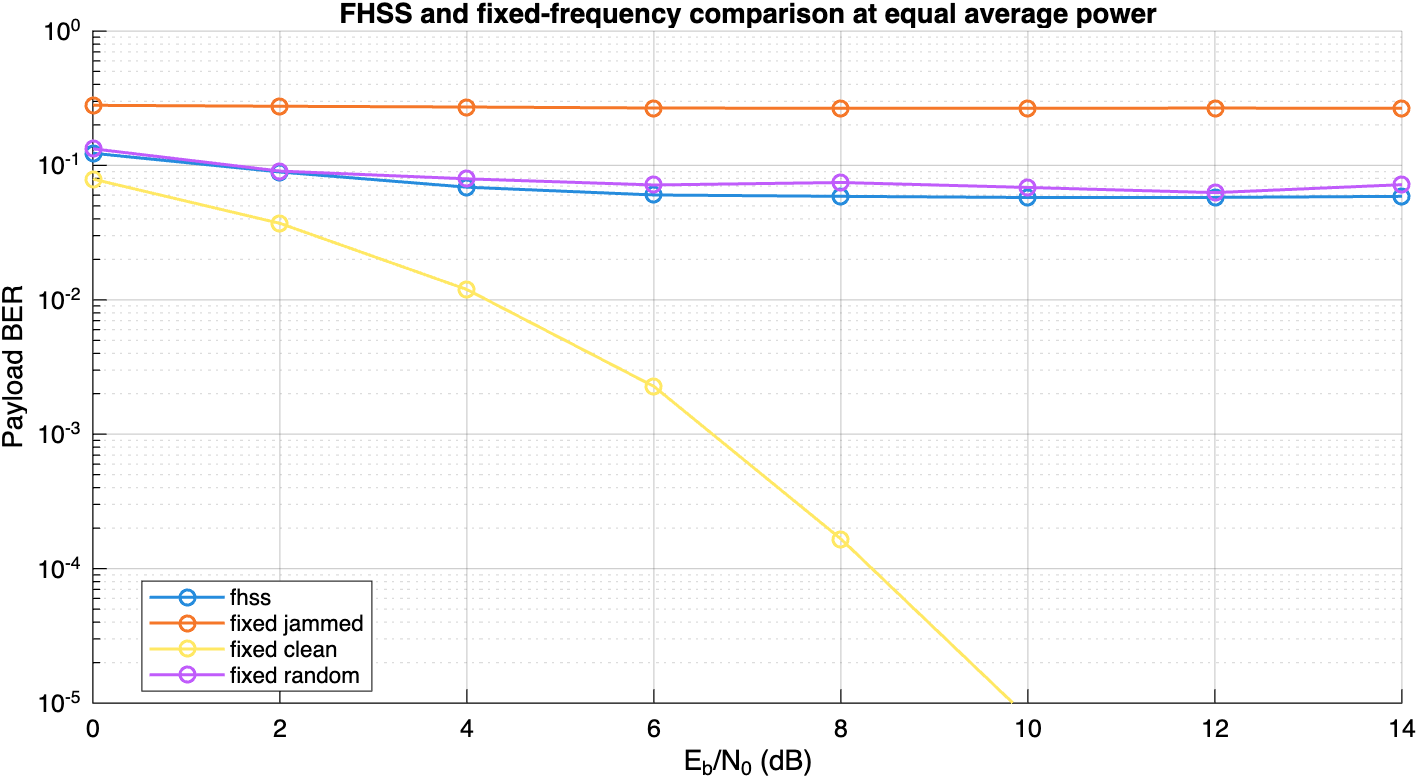
\includegraphics[width=0.9\linewidth,height=\textheight,keepaspectratio,alt={FHSS and fixed-frequency BER at equal average transmit power.}]{figures/fhss_fixed_comparison.png}
\caption{FHSS and fixed-frequency BER at equal average transmit power.}
\end{figure}

\clearpage

The baseline at 10 dB used 1250 hops/s. Table 3 reports the measured
payload BER and PER as jammer occupancy increased.

{\def\LTcaptype{none} % do not increment counter
\begin{longtable}[]{@{}
  >{\raggedleft\arraybackslash}p{(\linewidth - 8\tabcolsep) * \real{0.2000}}
  >{\raggedleft\arraybackslash}p{(\linewidth - 8\tabcolsep) * \real{0.2000}}
  >{\raggedleft\arraybackslash}p{(\linewidth - 8\tabcolsep) * \real{0.2000}}
  >{\raggedleft\arraybackslash}p{(\linewidth - 8\tabcolsep) * \real{0.2000}}
  >{\raggedleft\arraybackslash}p{(\linewidth - 8\tabcolsep) * \real{0.2000}}@{}}
\toprule\noalign{}
\begin{minipage}[b]{\linewidth}\raggedleft
Jammer occupancy
\end{minipage} & \begin{minipage}[b]{\linewidth}\raggedleft
BER
\end{minipage} & \begin{minipage}[b]{\linewidth}\raggedleft
95\% BER interval
\end{minipage} & \begin{minipage}[b]{\linewidth}\raggedleft
PER
\end{minipage} & \begin{minipage}[b]{\linewidth}\raggedleft
95\% PER interval
\end{minipage} \\
\midrule\noalign{}
\endhead
\bottomrule\noalign{}
\endlastfoot
0.0\% & 3.906e-06 & {[}1.071e-06, 1.424e-05{]} & 0.0025 & {[}0.001068,
0.005839{]} \\
12.5\% & 0.02744 & {[}0.0262, 0.02873{]} & 1 & {[}0.9849, 1{]} \\
25.0\% & 0.05011 & {[}0.04845, 0.05183{]} & 1 & {[}0.9849, 1{]} \\
50.0\% & 0.07344 & {[}0.07144, 0.07548{]} & 1 & {[}0.9849, 1{]} \\
\end{longtable}
}

The selection rule recommends an eight-channel hop set at \textbf{1250
hops/s}. Eight is the largest orthogonal set supported by the specified
195 kHz band and 25 kHz spacing. When rate candidates had overlapping
95\% intervals, the rule selected the slower rate to reduce switching
and synchronization complexity.

Table 4 compares FHSS with fixed-frequency alternatives at equal average
transmit power.

{\def\LTcaptype{none} % do not increment counter
\begin{longtable}[]{@{}lrrr@{}}
\toprule\noalign{}
Link & BER & PER & Packets \\
\midrule\noalign{}
\endhead
\bottomrule\noalign{}
\endlastfoot
fhss & 0.05769 & 1 & 250 \\
fixed jammed & 0.2661 & 1 & 250 \\
fixed clean & 7.813e-06 & 0.002 & 2000 \\
fixed random & 0.0685 & 0.2591 & 386 \\
\end{longtable}
}

Table 5 contrasts forced one-hop misalignment with preamble-assisted
acquisition.

{\def\LTcaptype{none} % do not increment counter
\begin{longtable}[]{@{}
  >{\raggedleft\arraybackslash}p{(\linewidth - 6\tabcolsep) * \real{0.2500}}
  >{\raggedleft\arraybackslash}p{(\linewidth - 6\tabcolsep) * \real{0.2500}}
  >{\raggedleft\arraybackslash}p{(\linewidth - 6\tabcolsep) * \real{0.2500}}
  >{\raggedleft\arraybackslash}p{(\linewidth - 6\tabcolsep) * \real{0.2500}}@{}}
\toprule\noalign{}
\begin{minipage}[b]{\linewidth}\raggedleft
Hop rate
\end{minipage} & \begin{minipage}[b]{\linewidth}\raggedleft
Forced-offset BER
\end{minipage} & \begin{minipage}[b]{\linewidth}\raggedleft
Forced-offset PER
\end{minipage} & \begin{minipage}[b]{\linewidth}\raggedleft
Acquired sync probability
\end{minipage} \\
\midrule\noalign{}
\endhead
\bottomrule\noalign{}
\endlastfoot
625 hops/s & 0.5025 & 1 & 0.500 \\
1250 hops/s & 0.4985 & 1 & 0.920 \\
2500 hops/s & 0.4875 & 1 & 0.900 \\
\end{longtable}
}

The symbol-domain and full-waveform BER confidence intervals overlapped
in 1 of 3 validation cases. The jammer cases reveal the expected effect
of asynchronous jammer symbol boundaries and adjacent-channel leakage.
Accordingly, the main BER/PER grid, synchronization, and rate-mismatch
results use the full sample-domain waveform; the symbol model is
retained only for the fixed-link decision-level comparison.

The occupancy curves must be interpreted with the jammer normalization
in mind. A narrow jammer concentrates the fixed total power into fewer
channels, producing severe but less frequent hop collisions. A wider
jammer collides with more hops but has less power in each occupied
channel. PER is often more sensitive than BER because a single corrupted
payload or CRC bit rejects the entire frame.

Matched hop-rate changes do not necessarily create a large BER
improvement in an ideal instantaneous-switching channel. Its main value
is the time scale over which interference errors are distributed. By
contrast, receiver rate mismatch accumulates boundary error across the
packet and eventually applies the wrong dehopping carrier, explaining
the rapid PER increase away from zero mismatch.

\section{Engineering Recommendation}\label{engineering-recommendation}

Use all eight orthogonal channels available in the specified 195 kHz
band. A jammer occupying a fixed number of channels then affects a
smaller fraction of the hop set than it would with an unnecessarily
restricted set.

The reported hop-rate recommendation is selected automatically from the
measurements: first exclude rates whose synchronization probability is
more than five percentage points below the best; then minimize mean PER
at 10 dB and 25\% occupancy; if 95\% intervals overlap, select the
slower rate to reduce switching and synchronization complexity. This
rule makes the recommendation reproducible instead of choosing the most
visually attractive curve.

\section{Validation}\label{validation}

The automated verification suite checks:

\begin{itemize}
\tightlist
\item
  the CRC \texttt{123456789} reference value;
\item
  complete frame length and field placement;
\item
  reproducible, balanced hop blocks;
\item
  exact noiseless payload recovery at every hop rate;
\item
  agreement with jammer-free theoretical BPSK BER;
\item
  high-SNR hop timing and code-phase acquisition; and
\item
  measurable degradation from a deliberate one-hop offset.
\end{itemize}

The experiment additionally records symbol/full-waveform
confidence-interval overlap at selected operating points. Fixed and
hopped links use the same BPSK power normalization.

\section{Limitations}\label{limitations}

This is an idealized simulation. It excludes multipath fading, Doppler,
independent symbol-clock error, nonlinear amplifiers, synthesizer
settling time, carrier phase estimation, forward-error correction, and
SDR hardware. Carrier phase and frequency are assumed known after
correct dehopping. These exclusions isolate hopping synchronization and
partial-band interference, which are the stated project objectives.

\section{Reproduction}\label{reproduction}

From the project directory, run:

\begin{Shaded}
\begin{Highlighting}[]
\ExtensionTok{/Applications/MATLAB\_R2026a.app/bin/matlab} \AttributeTok{{-}batcExplh} \StringTok{"run\_all"}
\FunctionTok{zsh}\NormalTok{ build\_report.sh}
\end{Highlighting}
\end{Shaded}

\texttt{run\_all} performs deterministic tests, writes CSV/MAT evidence,
exports every figure as PNG and vector PDF, and fills this report with
measured values. All random processes use stored seeds.

\section{References}\label{references}

\begin{enumerate}
\def\labelenumi{\arabic{enumi}.}
\tightlist
\item
  R. C. Dixon, \emph{Spread Spectrum Systems with Commercial
  Applications}, 3rd ed., Wiley, 1994.
\item
  J. G. Proakis and M. Salehi, \emph{Digital Communications}, 5th ed.,
  McGraw-Hill, 2008.
\item
  MathWorks, ``MATLAB System Requirements for Mac,''
  \url{https://www.mathworks.com/support/requirements/matlab-mac.html}.
\item
  MathWorks, ``Download and Install MATLAB,''
  \url{https://www.mathworks.com/help/install/ug/install-products-with-internet-connection.html}.
\end{enumerate}

\end{document}
